\section{Website Aufbau}
\frame{
    \frametitle{Website Aufbau}
    \begin{itemize}
        \item Startseite
        \item Studentinnen- \& Studentenrat
        \item weitere studentische Gremien
        \item Studentische Vertretung (an unserer Hochschule)
        \item Mitmachen
        \item Intern
        \item Hochschule
        \item Refugees Welcome
    \end{itemize}
}

\subsection{Startseite}
\frame{
    \frametitle{Website Aufbau - Startseite}
    \begin{figure}[!h]
        \centering
        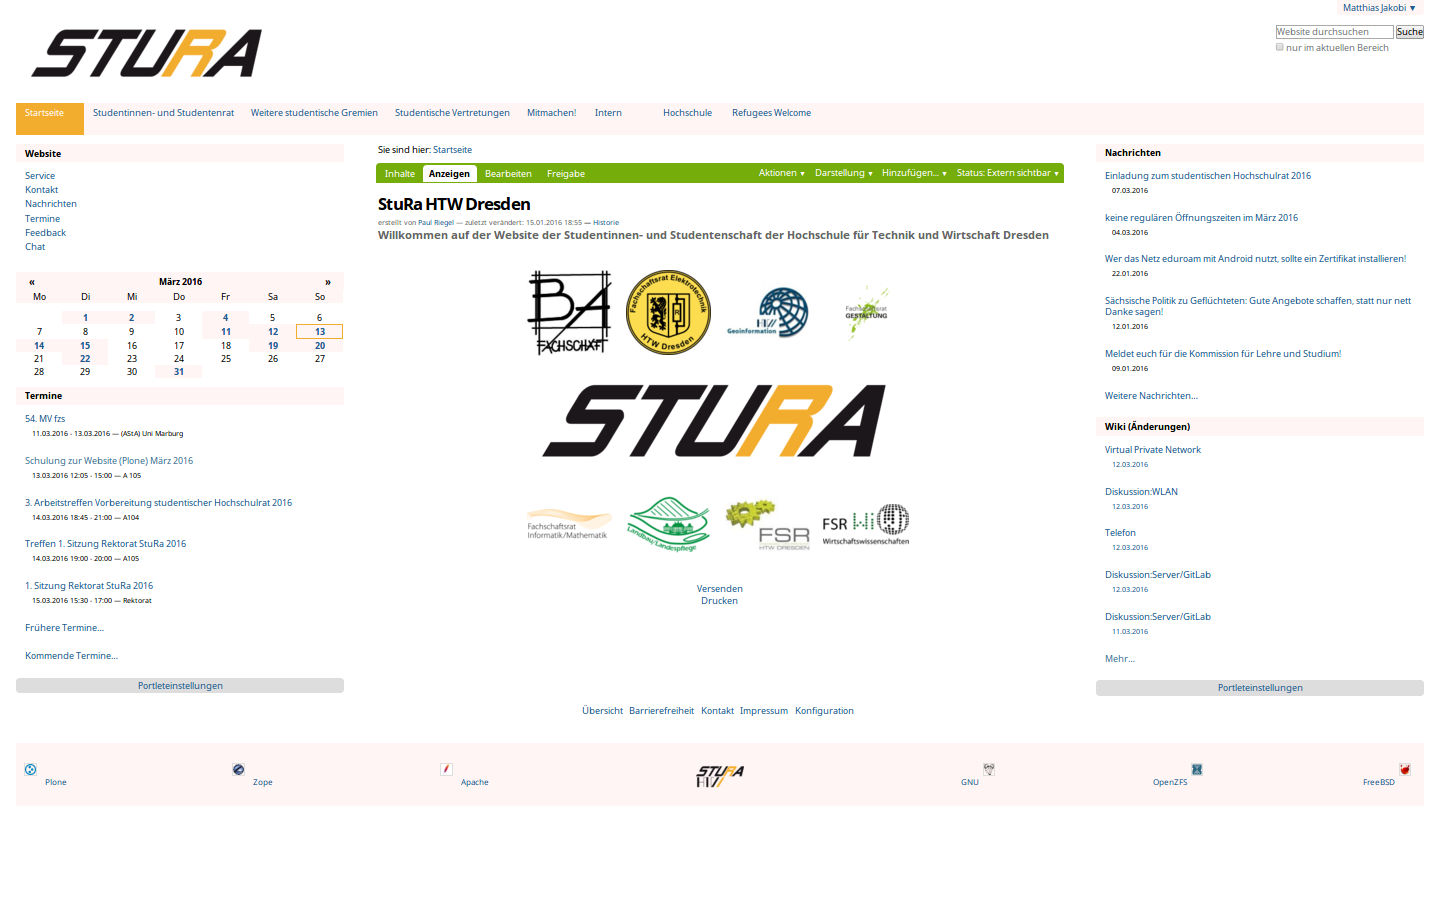
\includegraphics[width=0.9\textwidth]{../res/stura-startseite.png}
        \vspace{-20pt}
    \end{figure}
    \begin{itemize}
        \item aktuelle Inhalte
        \begin{itemize}
            \item Nachrichten
            \item Termine
            %\item Wikieinträge
        \end{itemize}
    \end{itemize}
}

\subsection{Studentinnen- \& Studentenrat}
\frame{
    \frametitle{Website Aufbau - Studentinnen- \& \newline Studentenrat}
    \begin{itemize}
        \item Übersicht, Struktur des StuRa
        \begin{itemize}
            \item Referate $\rightarrow$ Bereiche
            \item Sprecher*innen
            \item Referatskollegium
        \end{itemize}
    \end{itemize}
    \begin{itemize}
        \item allgemeines
        \begin{itemize}
            \item Sitzungen $\rightarrow$ Anträge $\rightarrow$ Protokolle
            \item Ordnungen
            \item Mitglieder
            \item Nachrichten
            \item Termine
        \end{itemize}
    \end{itemize}
}

\subsection{weitere studentische Gremien}
\frame{
    \frametitle{Website Aufbau - weitere studentische\newline Gremien}
    Ebenen: intern, lokal, regional, bundesweit, international
    \begin{itemize}
        \item Fachschaften
        \item Ausschüsse
        \item studentischer Hochschulrat
        \item Konferenz Sächsischer Studierendenschaften (KSS)
        \item freier zusammenschluss von studentinnenschaften (fzs)
        \item Studentischer Akkreditierungspool
    \end{itemize}
}

\subsection{Studentische Vertretungen}
\frame{
    \frametitle{Website Aufbau - Studentische Vertretungen}
    Ebenen: intern, lokal, regional, bundesweit, international
    \begin{itemize}
        \item Fakultätsräte
        \item Senat
        \item Erweiterter Senat
        \item Wahlausschuss HTW Dresden
        \item Verwaltungsrat Studentenwerk
        \item Unterstüzung
    \end{itemize}
}

\subsection{Mitmachen, Intern, Hochschule, Refugees Welcome}
\frame{
    \frametitle{Website Aufbau - Mitmachen, Intern,\newline Hochschule, Refugees Welcome}
    \begin{description}
        \item[Mitmachen] Übersicht der Stellausschreibungen
        \item[Intern] nur für angemeldete Nutzer*innen sichtbar;
            Daten, die nur StuRa-Mitgliedern zugänglich sein dürfen
        \item[Hochschule] Schnellverweis auf die Webseite der HTW Dresden
        \item[Refugees Welcome] Schnellverweis auf ein Antidis-Projekt
    \end{description}
}
